\documentclass[tikz, border=5mm]{standalone}
\usetikzlibrary{calc, positioning}
\usepackage{textcomp}
\tikzset{
% every node/.style={
% rectangle,
% draw,
% minimum width=2cm,
% minimum height=1.5cm
% },
% >=latex,
}

\begin{document}
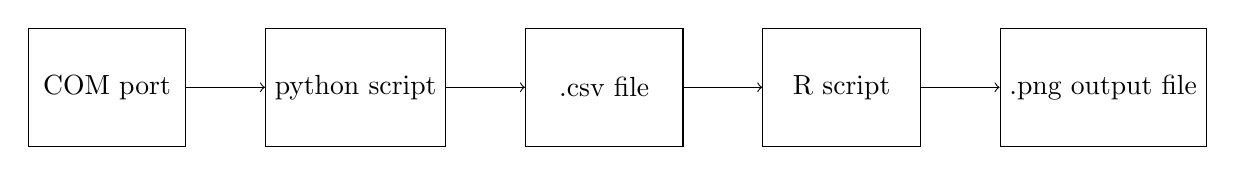
\begin{tikzpicture}[node distance=0.3cm and 1cm]

    % Nodes
    \node (a0) [              align=center, draw, minimum width=2cm, minimum height=1.5cm] {COM port};
    \node (a1) [right=of a0, align=center, draw, minimum width=2cm, minimum height=1.5cm] {python script};
    \node (a2) [right=of a1, align=center, draw, minimum width=2cm, minimum height=1.5cm] {.csv file};
    \node (a3) [right=of a2, align=center, draw, minimum width=2cm, minimum height=1.5cm] {R script};
    \node (a4) [right=of a3, align=center, draw, minimum width=2cm, minimum height=1.5cm] {.png output file};

    % Connectors
    \begin{scope}[->]

        \draw [->] (a0) -- (a1);
        \draw [->] (a1) -- (a2);
        \draw [->] (a2) -- (a3);
        \draw [->] (a3) -- (a4);

    \end{scope}

\end{tikzpicture}
\end{document}
